\section{Experiments}\label{sec:model}
In this section, we explain the design and parameters of all experiments conducted in this
research. The number of experiments is the cross product of data representation parameters and
network configuration parameters.


\subsection{Data Representation Parameters}\label{sec:param-data-repr-1}
For Arabic dataset representation, there are three parameters: \textit{diacritics} (2 values),
\textit{trimming} (2 values), and \textit{encoding} (3 values); and hence there are 12 different
data representations (the $x$-axis of Figure~\ref{fig:ArabicModelsResults}). A poem can be fed to the
network with/without \textit{diacritics} (1D/0D for short); this is to study their effect on
network learning. It is anticipated that it will be much easier for the network to learn with
\textit{diacritics} since it provides more information on pronunciation and phonetics. Arabic poem
data, as indicated in Figure~\ref{fig:footn-footn-class}-a, is not balanced. To study the effect of
this unbalance, the dataset is used once with \textit{trimming} the smallest 5 meters from the
dataset and once in full (no trimming), i.e., with all 16 meters presented (1T and 0D for
short). There are three different \textit{encoding} methods, \textit{one-hot}, \textit{binary}, and
\textit{two-hot} (OneE, BinE, TwoE for short), as explained in
Sec.~\ref{sec:data-encoding}. Although all carry the same information, it is expected that a
particular encoding may be suitable for the complexity of a particular network configuration. (see
Sec.~\ref{sec:discussion} for elaboration).

For English dataset representation, there is no \textit{diacritics} and the dataset does not suffer
a severe imbalance (Figure~\ref{fig:footn-footn-class}-a). Therefore, there are just 2 different
data representations, corresponding solely to \textit{one-hot} and \textit{binary} encodings (the
$x$-axis of Figure~\ref{english_results}-a).


\subsection{Network Configuration Parameters}\label{sec:param-netw-conf}
The main Recurrent Neural Network (RNN) architectures experimented in this research are: the Long
Short Term Memory (LSTM) introduced in~\cite{Hochreiter1997LongShortTermMemory}, the Gated Recurrent
Unit (GRU)~\citep{Cho2014LearningPhraseRepresentationsUsing}, and their bidirectional variants
Bi-LSTM and Bi-GRU\@. Conceptually, GRU is almost the same as the LSTM; however, GRU has less
architectural complexity, and hence a fewer number of training parameters. From benchmarks and
literature results, it is not clear which of the four architectures is the overall winner. However,
for their comparative complexity, it can be anticipated that both LSTM and Bi-LSTM (will be always
written as (Bi-)LSTM for short) may be more accurate than their two counterparts (Bi-)GRU on much
larger datasets and vice-versa.

\begin{figure}[!tb]
  \centering
  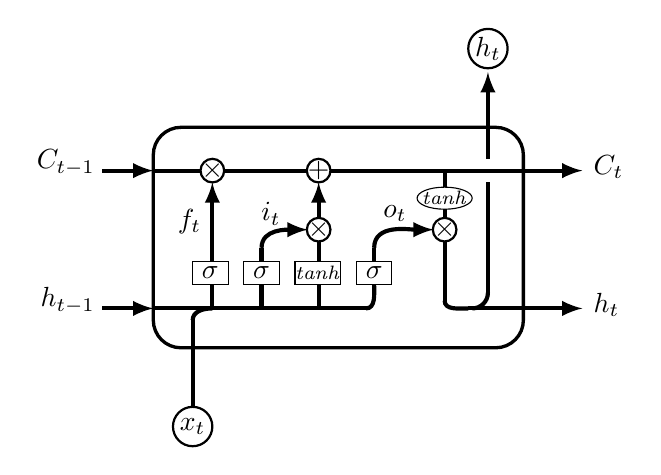
\begin{tikzpicture}

  % The grid
  % \draw[step=0.5, gray!40, very thin] (0,0) grid (8,4);

  % LSTM frame
  \def \yONE {0.5}
  \def \yTWO {3.3}
  \draw[rounded corners=10pt, very thick]  (1.5, 0.5) rectangle (6.2, 3.3);

  \def \sigmoidWidth  {0.45}
  \def \sigmoidInDist {0.2}
  \def \sigmoidHeight  {0.3}
  \def \yB  {1.3}
  \def \yD  {2.75}
  \def \shift {0.3}
  % First Sigmoid
  \draw  (2, \yB) rectangle (2+ \sigmoidWidth, \yB + \sigmoidHeight) node[pos=0.5] {$\sigma$};

  \def \r {.15cm}
  % The Upper times operator
  \draw[thick] (2.25, \yD) circle (\r) node {$\times$};

  % Second Sigmoid
  \def \xS {2.45 +\sigmoidInDist}
  \draw  (\xS, \yB) rectangle (\xS +\sigmoidWidth, \yB + \sigmoidHeight) node[pos=0.5] {$\sigma$};

  % Square tanh
  \def \xSS {\xS +\sigmoidWidth + \sigmoidInDist}
  \draw  (\xSS, \yB) 
  rectangle 
  (\xSS +\sigmoidWidth +0.13, \yB +\sigmoidHeight)
  node[pos=0.5] {\scriptsize \textit{tanh}};

  % Third Sigoid
  \def \xSSS {\xSS +\sigmoidWidth +0.13 +\sigmoidInDist}
  \draw  (\xSSS, \yB) rectangle (\xSSS +\sigmoidWidth, \yB +\sigmoidHeight)
  node[pos=0.5] { $\sigma$};

  % Second times operator and add operator
  \def \xTimesB {3.6}
  \def \yC      {2}

  \draw[thick] (\xTimesB, \yC) circle (\r) node {$\times$};
  \draw[thick] (\xTimesB, \yD) circle (\r) node {$+$};

  % Third times operator and its tanh
  \draw[thick] (\xTimesB +1.3 +\shift, \yC) circle (\r) node {$\times$};
  \draw (\xTimesB +1.3 +\shift, \yC +.4)  
  ellipse (.35cm and .14cm) 
  node {\scriptsize \textit{tanh}};


  % LINES
  \draw[arrows=-latex, line width=1.5pt]  (0.85, \yD) -- (1.5, \yD) 
  node[left, xshift=-.6cm, yshift=0.1cm] {$C_{t-1}$};
  \draw[line width=1.5pt]  (1.5, \yD) -- (2.1, \yD);
  \draw[line width=1.5pt]  (2.4, \yD) -- (3.46, \yD);
  \draw[arrows=-latex, line width=1.5pt]  (3.75, \yD) -- (6.75 +0.2, \yD)
  node[right, xshift=0.0cm, yshift=0.05cm] {$C_t$};

  \draw[arrows=-latex, line width=1.5pt]  (2.25, \yB +\sigmoidHeight) -- (2.25, 2.6)
  node[left, yshift=-0.5cm] {$f_t$};

  % Level B LINES
  \def \levelB {1}
  \draw[arrows=-latex, line width=1.5pt] (0.85, \levelB) -- (1.5, \levelB)
  node[left, xshift=-.6cm, yshift=0.1cm] {$h_{t-1}$};

  \draw[line width=1.5pt] (1.5, \levelB) 
  --
  (4.2, \levelB);

  \def \xOfThirdSigmoid {\xSSS + \sigmoidWidth/2}
  \draw[line width=1.5pt] (4.2, \levelB) to[out=0,in=270] (\xOfThirdSigmoid, \yB);

  % Third Sigmoid up line
  % END (\xTimesB +1.3 - 0.19 , \yC)
  \draw[line width=1.5pt] (\xOfThirdSigmoid, \yB + \sigmoidHeight) 
  --
  (\xOfThirdSigmoid, \yB + \sigmoidHeight + 0.17) ;

  \draw[arrows=-latex, line width=1.5pt] (\xOfThirdSigmoid, \yB + \sigmoidHeight+0.17) 
  to[out=90, in=180] 
  (\xTimesB +1.3 -0.14 +\shift , \yC) 
  node [left, yshift=0.2cm, xshift=-0.2cm] {$o_t$};

  % tanh line
  \draw [line width=1.5pt] (\xTimesB, \levelB)
  --
  (\xTimesB, \yB);

  \draw [line width=1.5pt] (\xTimesB, \yB + \sigmoidHeight)
  --
  (\xTimesB, \yB + \sigmoidHeight +0.24);

  \draw [arrows=-latex, line width=1.5pt] (\xTimesB, 2.15)
  --
  (\xTimesB, 2.6);

  \draw[line width=1.5pt] (2.25, \levelB)
  --
  (2.25, \yB);
  
  \draw[line width=1.5pt] (\xS +\sigmoidWidth/2, \levelB)
  --
  (\xS +\sigmoidWidth/2, \yB);

  \draw[line width=1.5pt] (\xS +\sigmoidWidth/2, \yB +\sigmoidHeight)
  -- 
  (\xS +\sigmoidWidth/2, \yB +\sigmoidHeight + 0.17);

  \draw[arrows=-latex, line width=1.5pt] (\xS +\sigmoidWidth/2, \yB + \sigmoidHeight+0.17) 
  to[out=90, in=180] 
  (\xTimesB-0.14, \yC)
  node [left, yshift=0.2cm, xshift=-0.2cm] {$i_t$};

  \def \bigR {0.25cm}
  \def \C    {1}
  \def \xBigCicleONE {2}
  \def \xBigCicleTWO {5.5 + 0.25}
  \draw[thick] (\xBigCicleONE, \yONE - \C) circle (\bigR) node {$x_t$};
  \draw[thick] (\xBigCicleTWO, \yTWO + \C) circle (\bigR) node {$h_t$};

  % LINE Circle ONE
  \draw[line width=1.5pt] (\xBigCicleONE, \yONE -\C +0.25) 
  --
  (\xBigCicleONE, \yONE -\C +0.25 + 1.1);

  \draw[line width=1.5pt] (\xBigCicleONE, \yONE -\C +0.25 + 1.1)
  to[out=90, in=180]
  (2.25, 1);

  % LINE third \times
  \draw[line width=1.5pt] (\xTimesB +1.3 +\shift, 1.1)
  --
  (\xTimesB +1.3 +\shift, \yC - 0.15);

  \draw[arrows=-latex, line width=1.5pt] (5.5, 1) 
  --
  (6.75 +0.2, 1)
  node[right, xshift=0.0cm, yshift=0.05cm] {$h_t$};


  \draw[line width=1.5pt] (\xTimesB +1.3 +\shift, 1.1)
  to[out=270, in=180]
  (5.5, 1);


  \draw[line width=1.5pt] (\xTimesB +1.3 +\shift, 2.14)
  --
  (\xTimesB +1.3 +\shift, 2.26);


  \draw[line width=1.5pt] (\xTimesB +1.3 +\shift, \yD)
  --
  (\xTimesB +1.3 +\shift, 2.54);


  \draw[line width=1.5pt] (\xBigCicleTWO, \levelB +0.2)
  --
  (\xBigCicleTWO, 2.6);

  \draw[line width=1.5pt] (\xBigCicleTWO - 0.2, \levelB)
  to[out=0, in=270]
  (\xBigCicleTWO, \levelB +0.2);


  \draw[arrows=-latex, line width=1.5pt]
  (\xBigCicleTWO, \yD +0.15)
  --
  (\xBigCicleTWO, 4);

\end{tikzpicture}

  \caption{Architecture of a single LSTM cell, the building block of LSTM RNN\@. (Figure adapted
    from~\cite{Colah2015UnderstandingLstmNetworks})}\label{lstm}
\end{figure}

We will give a very brief account for LSTMs, which was designed to solve the long-term dependency
problem. The other three architectures have the same design flavor and the interested reader can
refer to their literature. In theory, RNNs are capable of handling long-term dependencies. However,
in practice they do not, due to the \textit{exploding gradient} problem, where weights are updated
by the gradient of the loss function with respect to the current weights in each training epoch. In
some cases, the gradient may become infinitesimally small, which prevents weights from changing and
may stop the network from further learning. LSTMs are designed to be a remedy for this
problem. Figure~\ref{lstm} (adapted from~\cite{Colah2015UnderstandingLstmNetworks}) shows an LSTM
cell, where: $f_t$ is the forgetting gate, $i_t$ is the input gate, $o_t$ is the output gate, $C_t$
is the memory across cells, $W_j,\ U_j,\ b_j,\ j \in \left\{f, i, o\right\}$ are the weight matrices
and bias vector. The cell hidden representation $h_t$ of $x_t$ is computed as follows:%
\begin{align*}
  f_t  &= \sigma(W_f  x_t + U_f h_{t-1} + b_t),\\
  i_t  &= \sigma(W_i  x_t + U_i h_{t-1} + b_i),\\
  o_t  &= \sigma(W_o  x_t + U_o h_{t-1} + b_o),\\
  C_t  &= f_t \circ c_{t-1} + i_t \circ \tanh(W_c x_t + U_c h_{t-1} + b_c),\\
  h_t  &= o_t \circ \tanh(c_t).
\end{align*}

Next, we detail the network configuration parameters of all experiments. For Arabic dataset, there
are four parameters: \textit{cell} (2 values), \textit{layers} (2 values), \textit{size} (2
values), and \textit{weighting} (2 values). Therefore, there are $16$ different network
configurations to run on each of the 12 data representations above. This results in
$16 \times 12 (=192)$ different experiments (or models). For \textit{cell}, we tried both LSTM and
Bi-LSTM\@. Ideally, GRU and Bi-GRU should be experimented as well. However, this would require
almost the double of execution time, which would not be practical for the research life time. This
is deferred to another large scale comprehensive research currently running
(Sec.~\ref{sec:discussion}). We tried 4 and 7 \textit{layers}, with internal vectorized
\textit{size} of 50 and 82. Finally, another alternative to \textit{trimming} small classes (meters)
that was discussed above, in data representation parameters (Sec.~\ref{sec:param-data-repr-1}), is
to keep all classes but with \textit{weighting} the loss function to account for the relative class
size. For that purpose, we introduce the following \textit{weighting} function:%
\begin{align}
  w_c &= \frac{1/n_c}{\sum_{c'} 1/n_{c'}}, \label{eq:1}
\end{align}%
where $n_c$ is the sample size of class $c$, $c = 1, 2, \ldots C$, and $C$ is the total number of
classes (16 meters in our case).

For English dataset, there are four parameters: \textit{cell} (4 values), \textit{layers} (6
values), \textit{size} (4 values). We did not include \textit{weighting} since the dataset does not
suffer sever unbalance as is the case for the Arabic dataset. Therefore, there are $96$ different
network configurations to run on each of the 2 data representations above. This results in the same
number of 192 different experiments ($96 \times 2$) as those of the Arabic dataset. For
\textit{cell}, we had the luxury to experiment with the four types (Bi-)LSTM and (Bi-)GRU, since the
dataset is much smaller than the Arabic dataset. For \textit{layers}, we tried $3,4,\ldots, 8$, each
with internal vectorized \textit{size} of 30, 40, 50, and 60.

\bigskip

For all the 192 experiments on Arabic dataset and the 192 experiments on English dataset, networks
are trained using dropout of 0.2, batch size of 2048, with Adam optimizer, and 10\% for each of
validation and testing sets. Experiments are conducted on a Dell Precision T7600 Workstation with
Intel Xeon E5-2650 32x 2.8GHz CPU, 64GB RAM, 2 $\times$ NVIDIA GeForce GTX TITAN X (Pascal) GPUs;
and with: Manjaro 17.1.12 Hakoila OS, x86\_64 Linux 4.18.9-1-Manjaro Kernel.
